\section{Benchmarking the Analysis with Boosted Trees}\label{sec:XGBoost}
Boosted trees have been an essential part of \ac{HEP} analysis for many years (see 
\cite{ATLAS-CONF-2011-152} and \cite{ATLAS-CONF-2017-064}). The XGBoost framework has likewise 
been used as the benchmark for many \ac{ML} analysis, often chosen for its performance in sensitivity and 
extreme \ac{HPC} capabilities. Another reason for its popularity is the incredibly simple \ac{API}, allowing 
to create and predict a model in two lines of code. Additionally, its incredible boosting capabilities mean 
that it is little effected by variation in its structure. This leads many to the conclusion that the default 
parameters (see section \ref{subsec:XGBoost}) are often the best. 
\\
I choose to perform a sensitivity analysis for the original signal data set using a XGBoost model. The results
will act as a benchmark when performing further testing with \ac{NN}-variants. In figure \ref{fig:XGBoost} 
I have presented a grid displaying the achieved significance (see section \ref{subsec:Sensitivity}) for each 
mass combination in the original signal data set. In the figure we can observe that the XGBoost model performs
better for smaller masses. This results can be somewhat counterintuitive, due to signal with smaller masses 
having a larger resemblance to background than signal with large masses. The explanation is simply that there are
far more events with smaller masses than there are with larger mass. By studying figure \ref{fig:nrSignal} we know that 
there are a total of 134 events with ($\tilde{\chi}_1=200$, $\tilde{\chi}_2=400$GeV) compared to 6 events 
with ($\tilde{\chi}_1=400$, $\tilde{\chi}_2=800$GeV). Not only does this mean that the model will have had 
more small mass signal to train on than large mass, but also that a potential signal region would have to keep 
far more of the large mass signal to achieve a high significance.
\\
\begin{figure}
    \centering
    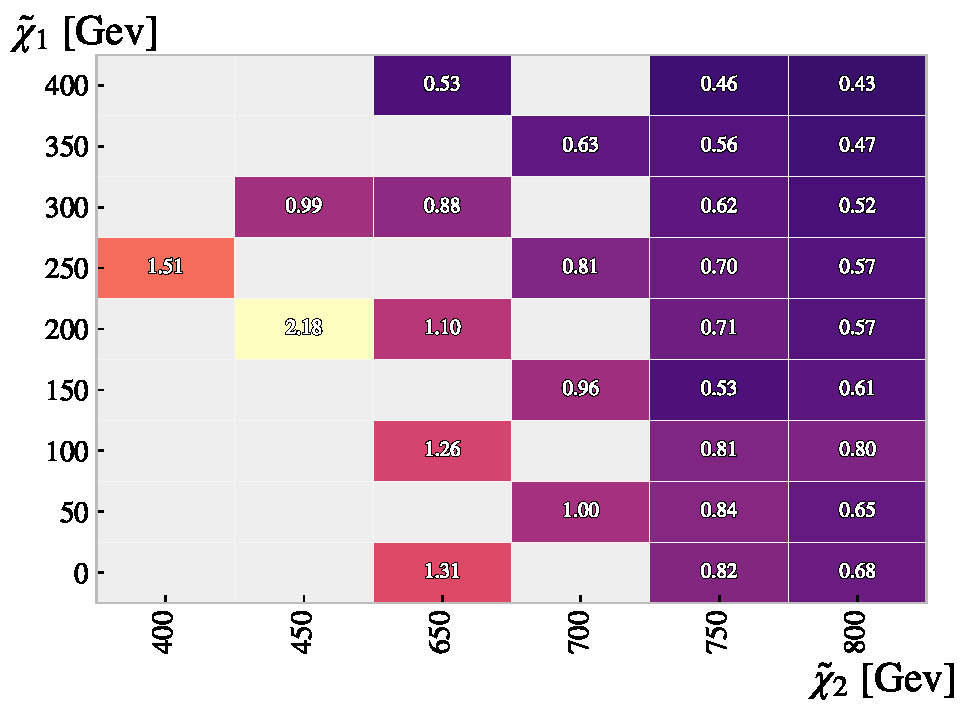
\includegraphics[width=0.7\textwidth]{Figures/MLResults/XGB/SUSY/Grid/XGBGridSig.pdf}
    \caption{A grid displaying the achieved significance on the original signal set, using the signal region 
    created by the \emph{XGBoost} network.}
    \label{fig:XGBoost}
\end{figure}
To further investigate the performance of the XGBoost model, I have drawn the distribution of the output for the 
entire background data set as well as for signal with 4 different mass combinations. The result is found in figure 
\ref{fig:XGBDistComp}. The figure shows the output of the XGBoost model with the full output range \ref{fig:XGBDist}
and the output ranging from [0.975-1.00]\footnote{This interval was chosen to study the higher output region.} (\ref{fig:XGBDist_95}). 
From the figure we observe a clear separation between 
signal and background, where most of the signal is give a high output ($>0.9$) and most of the background is given small
output ($<0.1$). To further support the effect of statistics in the signal, we can take note of the 
amount of signal in the higher range of the output (0.975-1). Although the model is able to achieve a much higher 
effectiveness (is able to preserve more of the signal) for higher mass signals, there are over 4 times as many 
events with mass ($\tilde{\chi}_1=200$, $\tilde{\chi}_2=400$GeV) (the lightest mass combination in the figure) then there 
are of any other.
\\
A final observation from figure \ref{fig:XGBDistComp}, is the study of which \ac{SM} processes contribute the most 
for higher model output. In figure \ref{fig:XGBDist_95}, we can see that in the output range of [$0.975-1$], the highest 
contributing processes are $Diboson(lll)$, $Top-Other$ and $t\bar{t}$. On the other hand $Z-jets$, which is originally the 
largest contributing processes, is almost removed in the higher output range. This aligns with my predictions made when studying the 
distribution of $E_T^{miss}$ (see section \ref{subsec:Validation}). 
\begin{figure}
    \makebox[\linewidth][c]{%
    \centering
    \hfill
    \begin{subfigure}{.6\textwidth}
        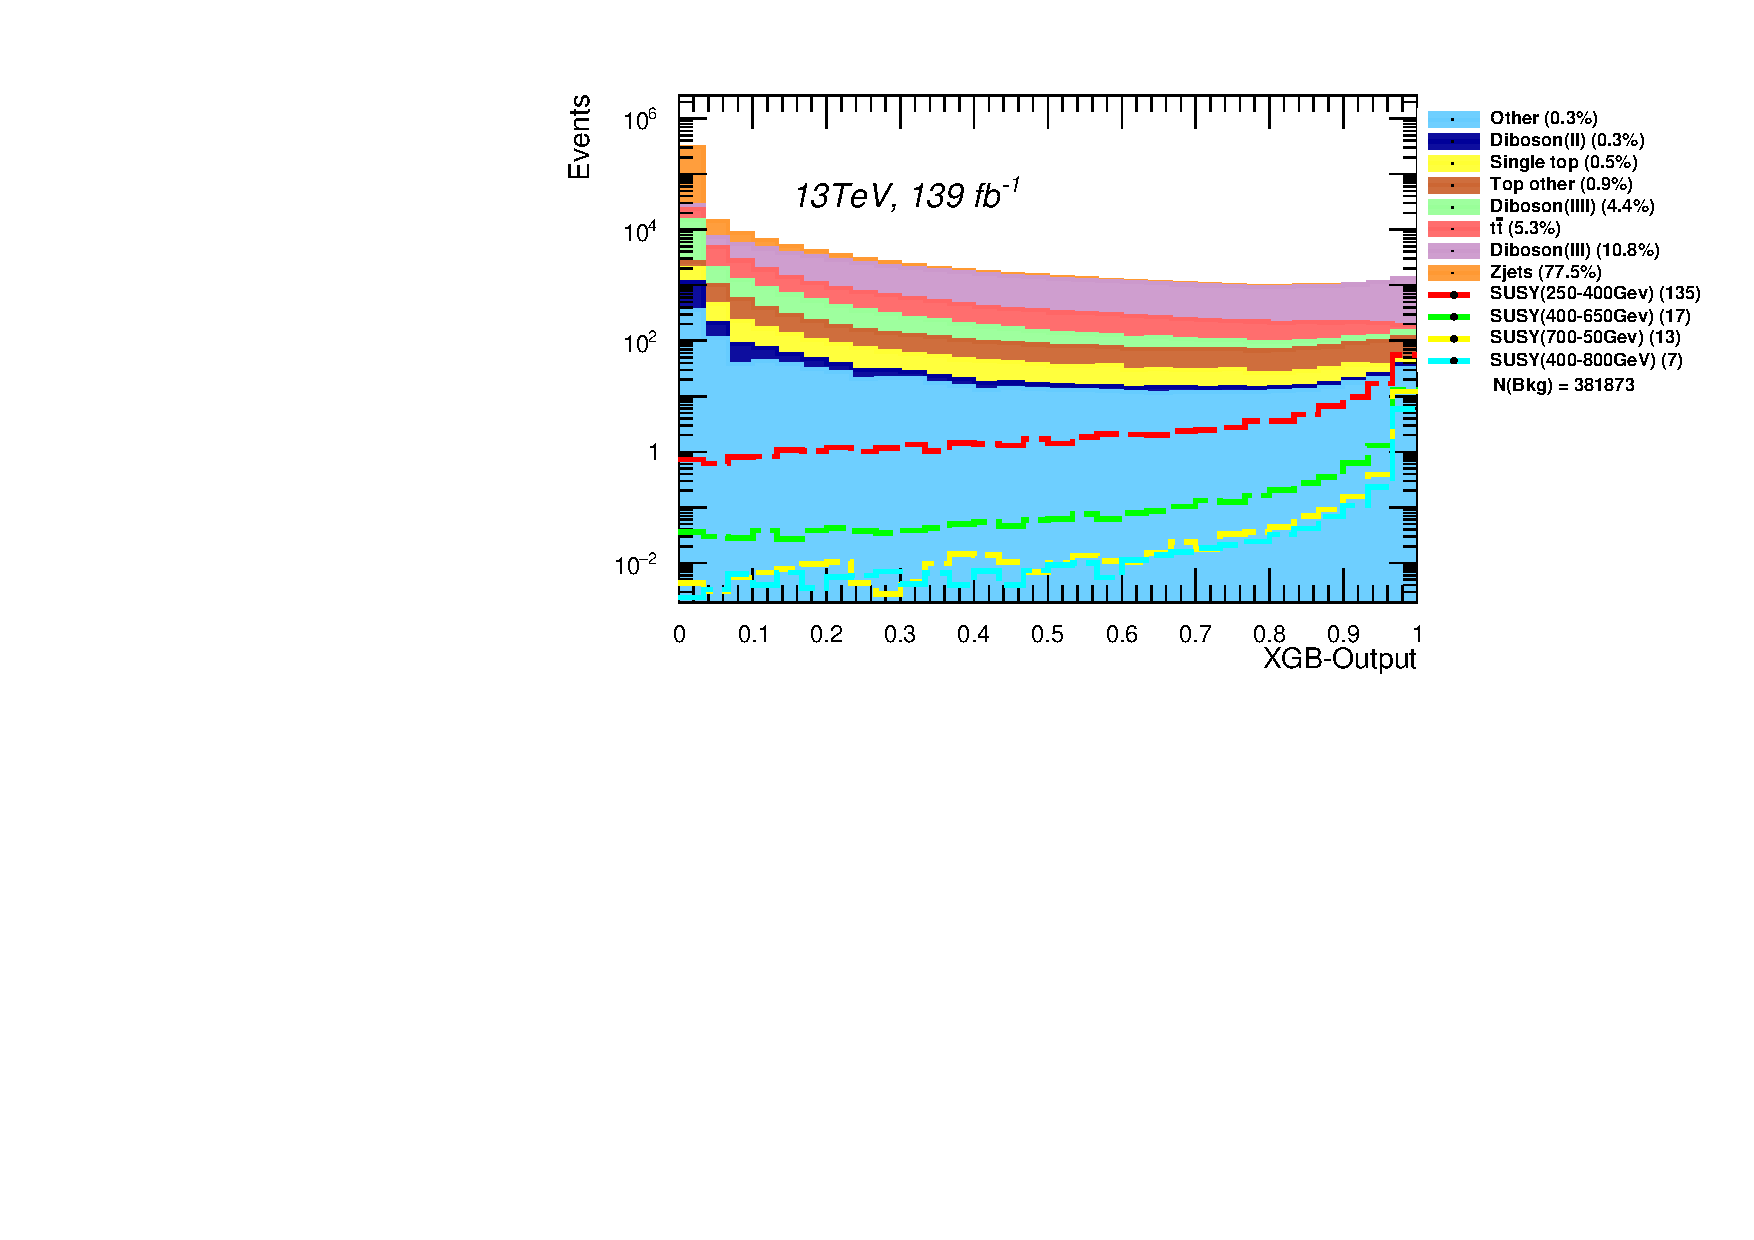
\includegraphics[width=\textwidth]{Figures/MLResults/XGB/SUSY/MLDist/xgbDist.pdf}
        \caption{}
        \label{fig:XGBDist}
    \end{subfigure}
    \begin{subfigure}{.6\textwidth}
        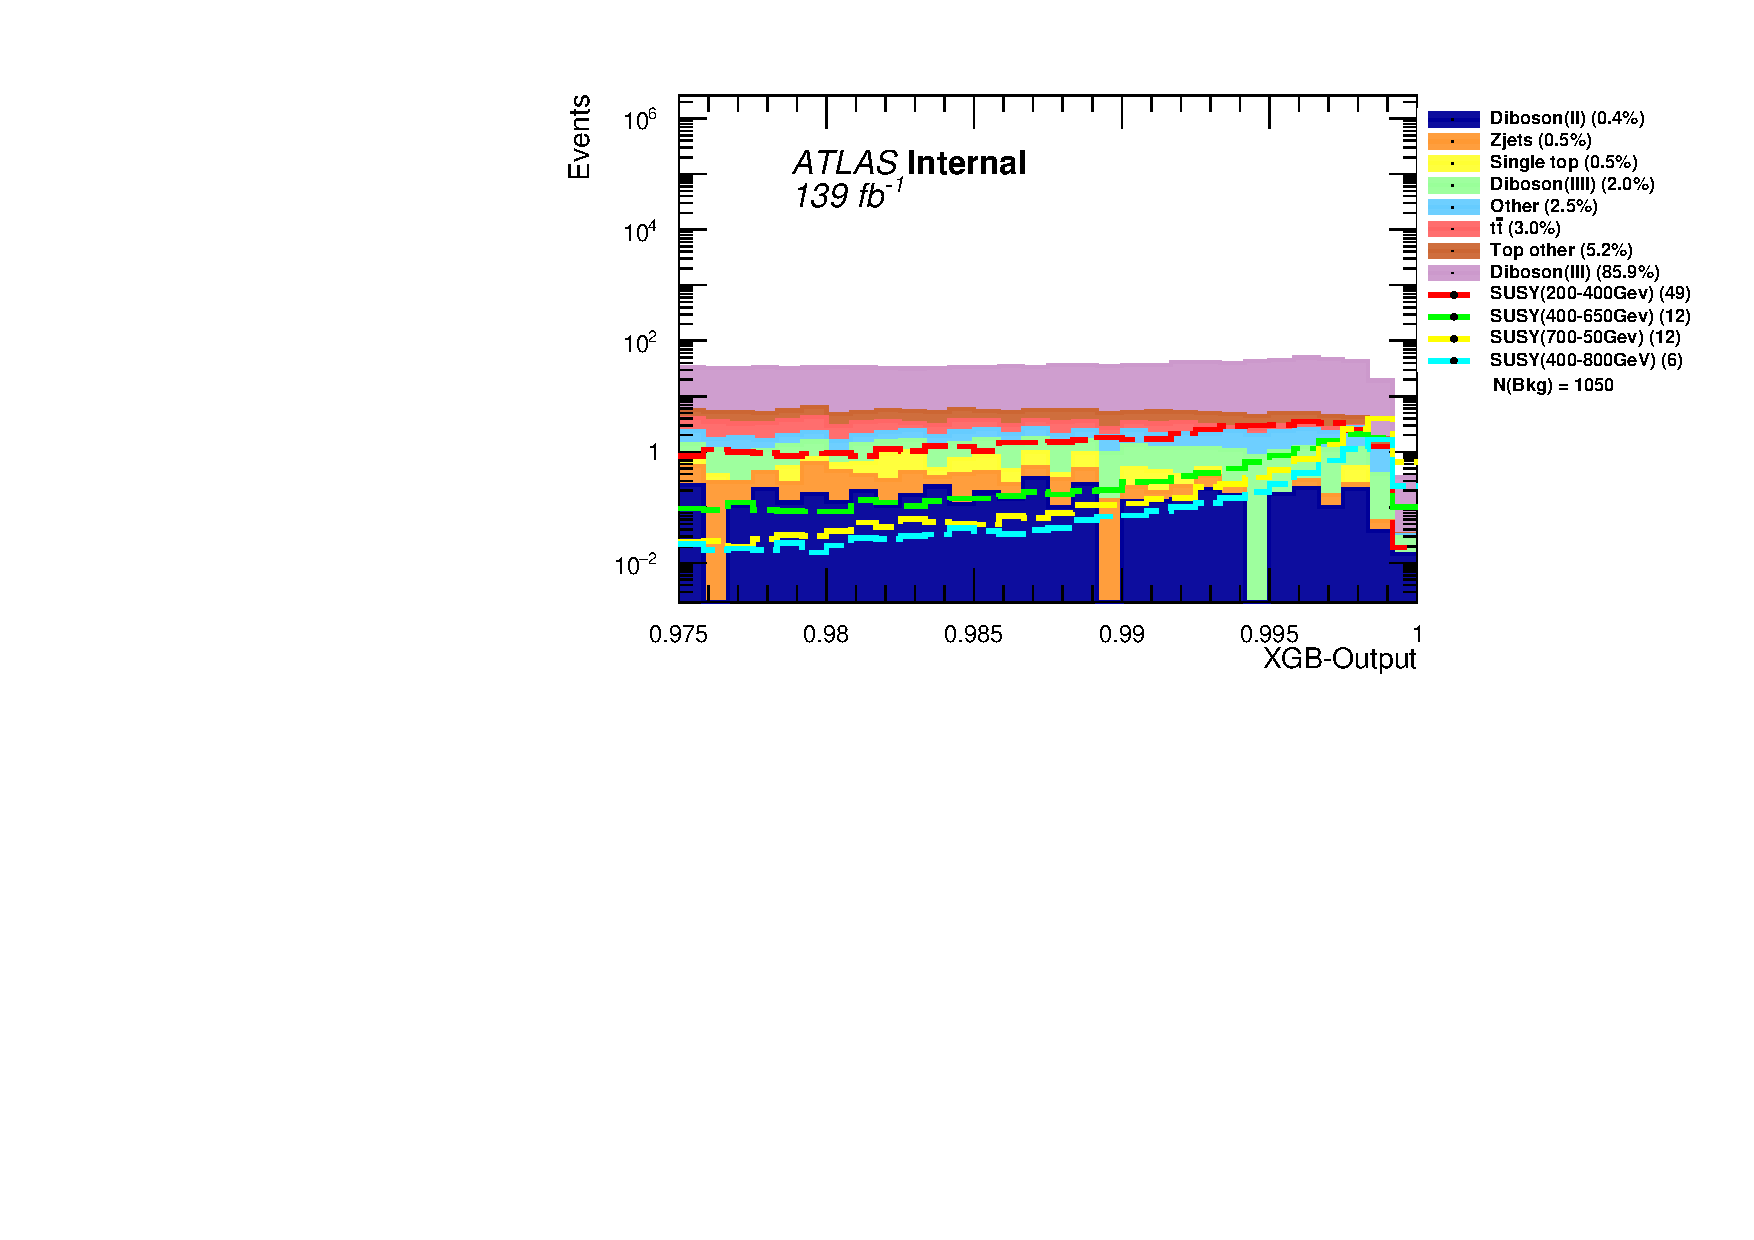
\includegraphics[width=\textwidth]{Figures/MLResults/XGB/SUSY/MLDist/xgbDist_C7.pdf}
        \caption{}
        \label{fig:XGBDist_95}
    \end{subfigure}
    \hfill
    }
    \caption{The output distribution from a trained XGBoost model for the background and signals with 4 different mass combinations:
    ($\tilde{\chi}_1=200$, $\tilde{\chi}_2=400$GeV), ($\tilde{\chi}_1=400$, $\tilde{\chi}_2=650$GeV), 
    ($\tilde{\chi}_1=700$, $\tilde{\chi}_2=50$GeV) and ($\tilde{\chi}_1=400$, $\tilde{\chi}_2=800$GeV). 
    The figure includes the full output range (\ref{fig:XGBDist}) and the output ranging from 0.9-1.00 (\ref{fig:XGBDist_95}).}
    \label{fig:XGBDistComp}
\end{figure}
